\chapter{MacroLab}
\label{sect:macrolab}

\emph{MacroLab} is a macroprogramming abstraction that provides a vector-based
syntax similar to Matlab~\cite{matlab}.  All data on nodes, including sensor
values, internal state, and parameters for actuation, are abstracted for the
user as vectors called \emph{macrovectors}.  The user can operate on
macrovectors with Matlab's standard set of vector operations such as {\tt max},
{\tt min}, {\tt sum}, or {\tt find}\footnote{Matlab's {\tt find} operator
returns the indices of non-zero elements in a vector}, and the system compiles
these down into local actions for each node that cooperatively execute the
vector operations.

MacroLab introduces a new data structure called a {\em macrovector} which can be
used to store in-network data such as sensor readings. Conceptually, each
element of a macrovector corresponds to a different node in the network, but
macrovectors can be stored in different ways. Each element can be on its
corresponding node, all elements can be on a central server, or all elements can
be replicated on all nodes.  No matter how a macrovector is stored, it can
support standard vector operations such as {\tt addition}, {\tt find}, and {\tt
max}.  These operations may run in parallel on a distributed macrovector,
sequentially on a centralized macrovector, or somewhere in between.  Thus, by
changing the representation of each macrovector, MacroLab can decompose a
macroprogram in the way that is most efficient for a particular deployment.  For
example, it may use centralized representations for small star topologies and
distributed representations in large mesh networks. This approach is called {\em
deployment-specific code decomposition (DSCD)}.

In contrast to systems like TinyOS~\cite{Levis}, the MacroLab programmer
specifies application logic in terms of abstract computation and does not need
to explicitly control data partitioning or message passing from within the
source code.  Instead, these tasks are performed automatically as compile-time
and run-time optimizations.  By separating application logic from program
decomposition, MacroLab can improve code portability, increase code reuse, and
decrease overall development costs.  Furthermore, it can reduce overall resource
consumption. The results show that automatically choosing a decomposition for
each deployment can reduce message passing by up to 50\% over using a single
decomposition for all deployments.

MacroLab provides a clear cost model so that the programmer can write
code that produces efficient and optimized decompositions.  This is
analogous to the idea in Matlab that vectorized code is more efficient
than {\tt for} loops.  MacroLab does not compromise on power or memory
efficiency in order to provide a high-level vector programming
abstraction and the results indicate that MacroLab programs are just
as efficient as normal TinyOS programs.

\section{Background and Related Work} \label{sect:relatedwork}

Macroprogramming systems have been proposed with a wide variety of abstractions
and programming models, each of which is designed to make programming easier for
some class of applications.  For example, database-like systems such as
TinyDB~\cite{Madden} and Cougar~\cite{Yao} allow the user to specify the desired
data using declarative SQL-like queries.  These systems are most suitable for
data collection applications where the desired data can be described with a
declarative query.  Several systems such as Hood~\cite{Whitehousea},
Regions~\cite{Welsh2004}, and Proto~\cite{Bachrach} are designed for spatial
applications and allow users to specify operations over groups, neighborhoods,
or regions in space.  Other systems such as Semantic Streams~\cite{Whitehouse},
Flask~\cite{Mainland}, and Regiment~\cite{Newton} allow users to specify global
operations in terms of {\em data streams} and {\em stream operators}.  These are
most suitable for defining a static set of long-running operations over streams
of sensor data. Logical rule-based systems such as RuleCaster~\cite{Bischoff},
DSN~\cite{Chu2006}, and Snlog~\cite{Chu2007} allow the user to define a global
objective in terms of system wide invariants that must be enforced at run-time.
MacroLab is perhaps most similar to imperative macroprogramming abstractions
like Marionette~\cite{Whitehouseb}, Pleiades~\cite{Kothari},
Kairos~\cite{Gummadi}, COSMOS~\cite{Awan}, and Tenet~\cite{Gnawali}.  These
systems support general-purpose programming with a traditional imperative
programming model. Vicaire et al. proposed the Bundles~\cite{vicaire2010bundle}
programming abstraction that address some issues inherent in CPSs that were not
tackled by other programming abstractions. These issues include the possibility
of CPSs being systems of systems where the subsystems exist across
administrative domains. Bundles provides an abstraction of a logical collection
of devices that can be used by different groups of people with different access
restrictions. Bundles also handles mobility within and across CPSs. MacroLab is
the first macroprogramming system for CPSs to provide vector programming, a
powerful and concise abstraction that already has wide adoption among scientists
and engineers.

He et al.~\cite{he2008essentia} present an architecture for wireless sensor
networks called Essentia where the 

Several existing systems allow users to write imperative programs that can then
be distributed across multiple processors for the purposes of high performance
computing.  These include High Performance Fortran (HPF)~\cite{Richardson},
Fortran D~\cite{Hiranandani}, and Split-C~\cite{Culler}.  The fundamental
difference between these approaches and MacroLab is their dependence on the user
to specify how the data and operations should be distributed. For example,
Fortran D uses the statments \texttt{decomposition}, \texttt{align}, and
\texttt{distribute} to specify how to execute a program on multiple processors.
In contrast, MacroLab programs do not specify how to map the computation onto
the network. In fact, the system will create a different mapping for each
network on which the program is executed.

Other systems such as MagnetOS~\cite{Liu}, Coign~\cite{Hunt}, and
J-Orchestra~\cite{Tilevich} can automatically decompose a program and distribute
it across a network in order to minimize network traffic.  Similar to MacroLab,
these systems use program profiling to tailor the decomposition to a specific
network topology.  In contrast to MacroLab, these systems decompose programs at
the {\em object level}.  MagnetOS and J-Orchestra break a program up at the
boundaries of Java objects and use Java RMI between segments of the program.
Coign requires programs to conform to Microsoft's Component Object Model (COM)
and breaks them up at the boundary of the COM objects.  MacroLab introduces
parallelism at the level of individual operations instead of at the level of
objects or software components.

Finally, many systems allow the user to specify parallel operations using
parallel data structures. SET Language (SETL)~\cite{Schonberg} provides
primitive operations such as set membership, union, intersection, and power set
construction, which can be applied in parallel to elements of {\em unordered
sets}. Starlisp (*Lisp) can apply vector operations such as vector addition and
multiplication over {\em Parallel Variables (PVARS)} which are vectors with one
element per processor.  Similarly, NESL allows parallel operations on {\em
sequences}. These are similar to MacroLab's parallel vector operations on {\em
macrovectors}. However, MacroLab goes beyond these systems by employing {\em
multiple} underlying representations of a macrovector.  Unordered sets, PVARS,
and sequences can only be decomposed in one way while macrovectors are
decomposed in one of many different ways depending on the topology over which
the program is executed. MacroLab is the first system that can perform
automatic, topology-specific decomposition on programs describing parallel
operations on parallel data structures.

\section{MacroLab Architecture}

MacroLab allows the user to write a single program that is simple, robust, and
manageable and then automatically decomposes it depending on the target
deployment.  A {\em program decomposition} is a specification of where data is
stored in the network and how messages are passed and computations are performed
in order to execute the program.  A macroprogram may be decomposed into {\em
distributed} operations for a large mesh network, where data is stored on every
node and network operations are performed in-network.  It could also be
decomposed into {\em centralized} operations for a small star topology, where
all data is collected to a central base station.  A program may also be
decomposed into many points on the spectrum between purely centralized or purely
distributed code.  The implementation could also use group-based data processing
or in-network aggregation.

MacroLab's overall architecture is depicted in Figure~\ref{fig:System}.  A
macroprogram (described in Section \ref{sect:abstraction}) is passed to the
decomposer (Section \ref{sect:decomposer}) which generates multiple
decompositions of the macroprogram.  Each decomposition is passed to the cost
analyzer (Section \ref{sect:costAnalyzer}) which calculates the cost of each
with respect to the cost profile of the target deployment. This cost profile
must be provided by the user and may include information such as the topology,
power restrictions, and descriptions of the radio hardware. The cost analyzer
chooses the best decomposition and passes it to the compiler and run-time system
(Section \ref{sect:RTS}) which converts the decomposition into a binary
executable and executes it.  While it executes, the program and the run-time
system continue to collect information about the cost profile of the deployment
and feed this information back to the cost analyzer.  If the cost profile
changes or if the cost profile at compile time was incomplete or incorrect, the
cost analyzer may decide to reprogram the network with a new decomposition.

The architecture of MacroLab is presented in~\ref{fig:System}. An alternative
implementation would be a compiler using the cost profile implementation to
produce the correct decomposition the first time, but it is conceptually easier
to enumerate all possible implementations and evaluate them.

The following subsections discuss the four components of MacroLab: the
programming abstraction, the decomposer, the cost analyzer, and the run-time
system.

\subsection{Abstraction} \label{sect:abstraction}

MacroLab provides a {\em vector programming} abstraction similar to Matlab. A
vector is a data structure containing values called {\em elements}
that are arranged in rows and columns.  For example,
\[ r = \left[ \begin{array}{ccc} a & b & c \\ d & e & f \\ g & h & i \end{array}
\right]\] is a 3 x 3 vector with 9 elements.  Vectors can be indexed by
dimension: the element in the second row and the third column of $r$ can be
selected with {\tt r(2,3)} resulting in $f$.  In MacroLab, like in Matlab, the
``{\tt :}'' is used to select an entire dimension.  For example, {\tt r(3,:)}
selects the 3rd element of the first dimension (rows) and the entire second
dimension (columns), namely {\tt [g~h~i]}.  Operations such as {\em vector
addition} and {\em vector multiplication} operate on the data structures. The
operation {\tt find(r==f)} produces the index of the element in $r$ that has the
value $f$, which is $[2,3]$.  In addition to standard vector programming,
MacroLab introduces three new concepts to facilitate software development for
CPSs: the macrovector, the dot-product index, and the neighborhood.  These
concepts are discussed in the next three subsections.


\subsubsection{The Macrovector}

MacroLab introduces a new data structure called the {\em macrovector}.
Macrovectors differ from traditional vectors in that each element of a
macrovector is associated with a particular node in the network.  Thus,
macrovectors are \emph{unordered} and are \emph{indexed by node ID}.  This
abstraction can be useful, for example, to store sensor readings. If {\tt light}
is a macrovector storing the light values of each sensor, then the operation
{\tt light(5)} would retrieve the light value of the sensor node with
$ID=5$. Since sensor node IDs may be non-sequential, the elements in a
macrovector do not form a strict sequence.  Macrovectors can have multiple
dimensions, but only a single dimension is indexed by node ID.  The other
dimensions are normal vectors indexed sequentially.  Macrovectors can be created
using the command \vspace{.1in}
\begin{center}
\ttfamily\small
\begin{verbatim}
light = Macrovector(<scope>, [length], [length], ...)
\end{verbatim}
\end{center}
\vspace{.1in} 
\noindent where the {\tt scope} of the macrovector is the set of nodes with
which the elements are associated.  This scope is a vector of node IDs and the
length of the first dimension will be the number of IDs.  The lengths of
subsequent dimensions must be given for a multi-dimensional macrovector. These
{\tt length}s are simply integer values indicating the size of each dimension.

Macrovectors support many standard Matlab vector operations such as {\tt
addition}, {\tt subtraction}, {\tt cross-product}, {\tt find}, {\tt max}, and
{\tt min}.  These operations can be combined to perform {\em macro} operations
that operate on data associated with many different sensor nodes.  For example,
the operation \vspace{.1in}
\begin{center}
\ttfamily\small
\begin{verbatim}
maxLight = max( light )
\end{verbatim}
\end{center}
\vspace{.1in}
will return the maximum light value in the network.  
The operation
\vspace{.1in}
\begin{center}
\ttfamily\small
\begin{verbatim}
brightNodes = find( light > mean(light))
\end{verbatim}
\end{center}
\vspace{.1in}
will return the IDs of nodes that have above-average light values.  
The operation
\vspace{.1in}
\begin{center}
\ttfamily\small
\begin{verbatim}
hotLight = light( find( temp > 100 ) )
\end{verbatim}
\end{center}
\vspace{.1in}
will return the light values on nodes where the {\tt temp} value is higher
than 100.  If these vectors were tables in TinyDB, this would be similar
to posing the SQL query
\vspace{.1in}
\begin{center}
\ttfamily\small
\begin{verbatim}
SELECT light WHERE temp > 100
\end{verbatim}
\end{center}
\vspace{.1in}

\begin{figure}
  \centering
  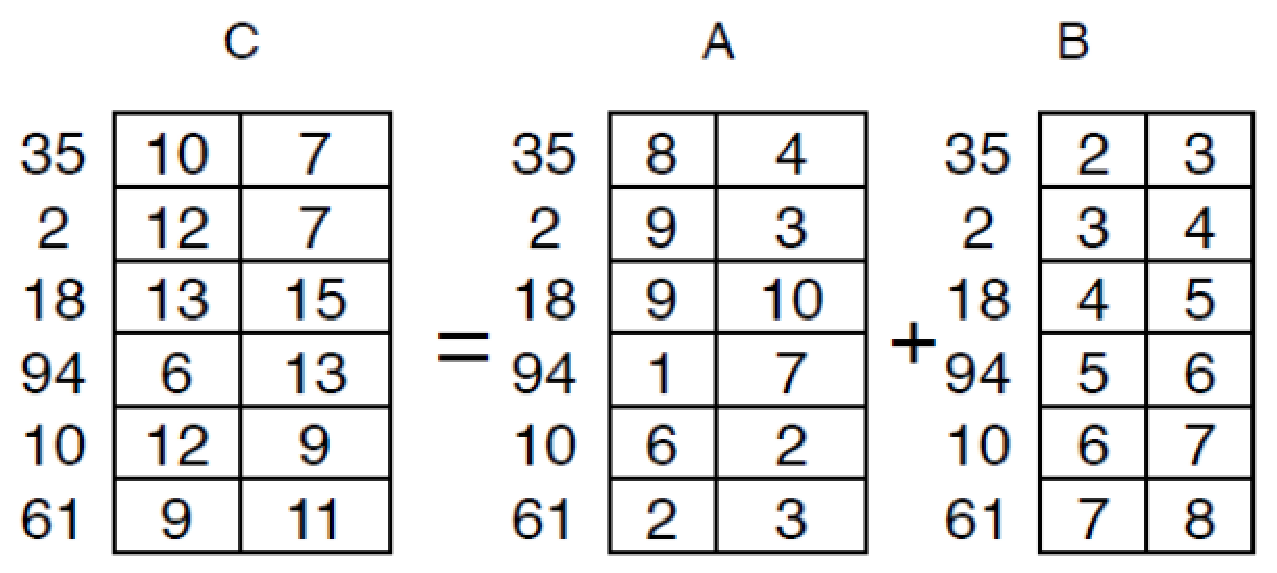
\includegraphics[width=0.6\columnwidth]{fig/DistributedArray1.eps}
  \caption[Example of a distributed macrovector]{Two $n \times 2$ macrovectors
  $A$ and $B$ can be added and stored into a third macrovector $C$. The values
  on the left of each vector indicate which node ID the cells are associated
  with.}
  \label{fig:macroVectorAddition}
\end{figure}

Elements associated with the same node ID are paired together for binary
operations that involve multiple macrovectors.  For example,
Figure~\ref{fig:macroVectorAddition} shows the operation {\tt C = A + B}
performed on three $n \times 2$ macrovectors. In this operation, the elements of
$A$ and $B$ corresponding to node $35$, for example, are added together and
stored in the elements of $C$ corresponding to node $35$.

\subsubsection{Dot-product Index} \label{sect:dotProduct} 

MacroLab provides a new way of indexing into macrovectors called the {\em
dot-product index}.  For example, with {\tt s~=~[1~2~3]} and {\tt t~=~[2~1~3]},
the aforementioned vector {\tt r} can be indexed as follows:
 \[ r(s,t)[1,2] == \left[ \begin{array}{ccc}
  & b &   \\
d &   &   \\
  &   & i \end{array} \right]\]

The two values in square brackets indicate that the elements of the first and
second dimension indices should be matched pair-wise before values are selected
from the matrix.  Since $s$ and $t$ each contain 3 elements, this dot-product
index would select 3 elements from $r$ in total.  With the values of $s$ and $t$
above, the dot-product index would select elements $[1, 2]$, $[2, 1]$, and $[3,
3]$.  This is different from traditional indexing in Matlab, which might be
called the {\em cross-product index}, in which the same index vectors would
produce
\[ r(s,t) = \left[ \begin{array}{ccc}
b & a & c \\
e & d & f \\
h & g & i \end{array} \right]\]

\begin{figure}[t]
  \centering
  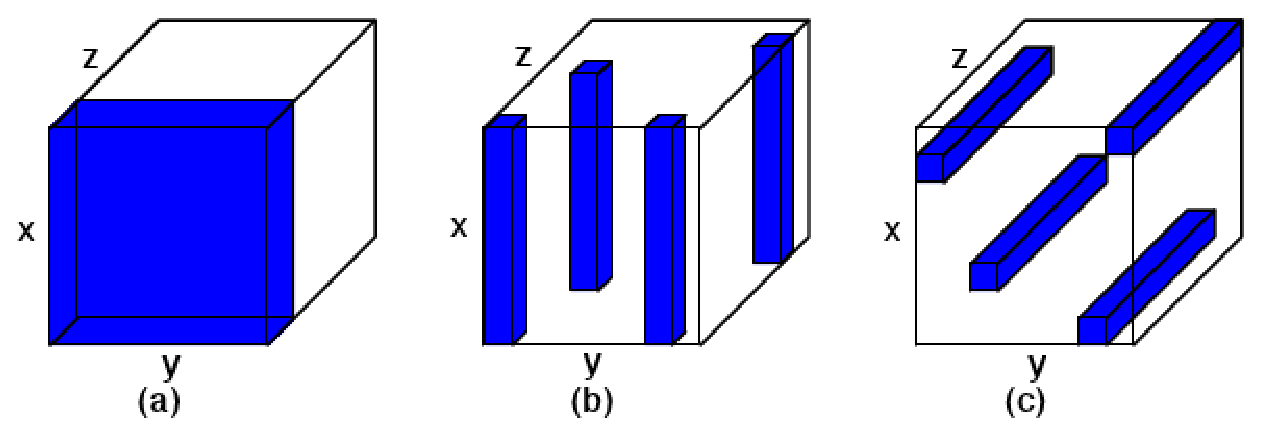
\includegraphics[width=0.8\columnwidth]{fig/DotProducts}
  \caption[Example of dot-product indexing]{A three-dimensional vector $D$ can
    be indexed with the (a) cross-product index {\tt D(x,y,1)}; (b) dot-product
    index {\tt D(:,y,z)[2,3]}; or (c) dot-product index {\tt D(x,y,:)[1,2]}.}
  \label{fig:dotProduct}
\end{figure}

In other words, all values of index vector $s$ are paired with all values of
index vector $t$, selecting 9 values in total.  Figure~\ref{fig:dotProduct}
illustrates how cross-products and dot-products can be used to select different
elements in a three-dimensional vector.

Dot-product indexing can be used to efficiently perform operations in which the
element to be selected on each node is different.  For example, if an $n \times
10$ macrovector {\tt circularBuffer} stored the last 10 light values read on
each node and an $n \times 1$ macrovector {\tt lastIndex} stored the index of
the most recent value stored, then the operation {\tt
circularBuffer(:,lastIndex)[1,2]} would provide the most recent value on each
node. The capabilities of macrovectors and dot-product indexing will be
demonstrated in Section~\ref{sect:evaluation}.

\subsubsection{Neighbor-based
Representation} \label{sect:neighborRepresentation} A node's {\em neighborhood}
is the set of nodes that are within radio range.  This is a very useful type of
{\em group} in which a node is guaranteed to have cheap communication to all
other nodes. Connectivity-based neighborhoods are often a critical part of
efficient in-network data processing algorithms.  Neighborhoods are a special
type of group since each node has a different neighborhood.  Because of this,
new syntax for defining a neighbor-based macrovector is introduced: 

\vspace{.1in}
\begin{center}
\ttfamily\small
\begin{verbatim}
lightReflection = neighborReflection(light)
\end{verbatim}
\end{center}
\vspace{.1in} 
\noindent which indicates that lightReflection is a vector of neighbor-based
macrovectors that should store {\em reflections} of the {\tt light}
macrovector. When a node writes to its own element of the {\tt light}
macrovector, that value is cached in the rows corresponding to its neighbors.
Thus, {\tt lightReflection} is a two dimensional vector where each row contains
cached values of a node's neighbors' light readings. Since each node may have a
neighborhood of different size, this is not necessarily a rectangular matrix;
each row may be a different length.  This abstraction is very similar to the
Hood programming abstraction~\cite{Whitehousea}.

\subsubsection{Program Decomposition} \label{sect:decomposer}

The MacroLab decomposer converts a macroprogram into a set of microprograms that
can be executed on nodes.  The goal is to preserve the semantics of the
macroprogram while allowing for efficient distributed operation.  The
decomposition algorithm has two steps. First, it chooses a data {\em
representation} for each macrovector, which can be {\em distributed}, {\em
centralized}, or {\em reflected} (Section~\ref{sect:decompositionTypes}).  Based
on the representations chosen, it then uses rule-based translation to convert
the vector operations in the macroprogram into network operations
(Section~\ref{sect:codeTranslation}).

\subsubsection{Choosing Macrovector Representations}\label{sect:decompositionTypes}

Macrovectors provide a uniform interface to several underlying {\em
representations}, which are different ways that the macrovector can be stored in
the network.  MacroLab currently supports three representations: distributed,
centralized, and reflected, the trade-offs of which are described in more detail
below.  Other representations are possible and would allow MacroLab to support
different classes of distributed algorithms.  Vector operations can be applied
to macrovectors regardless of their representation, making them ideally suited
for DSCD.

With three possible macrovector representations, a program with four
macrovectors would have $3^4$ possible decompositions.  Thus, the space of
decompositions grows exponentially with the number of macrovectors in a program.
Currently, MacroLab must systematically explore all possible combinations of
representations for the macrovectors in a program in order to find the optimal
decomposition.  This is currently not a problem for programs with only a small
number of macrovectors. For the programs described in this section, the
translation process from macrocode to microcode takes less than 0.5 seconds.  In
contrast, compilation of the microcode to a binary executable takes over 13
seconds, using the nesC and Matlab compilers.

\begin{figure}[h]
  \centering
  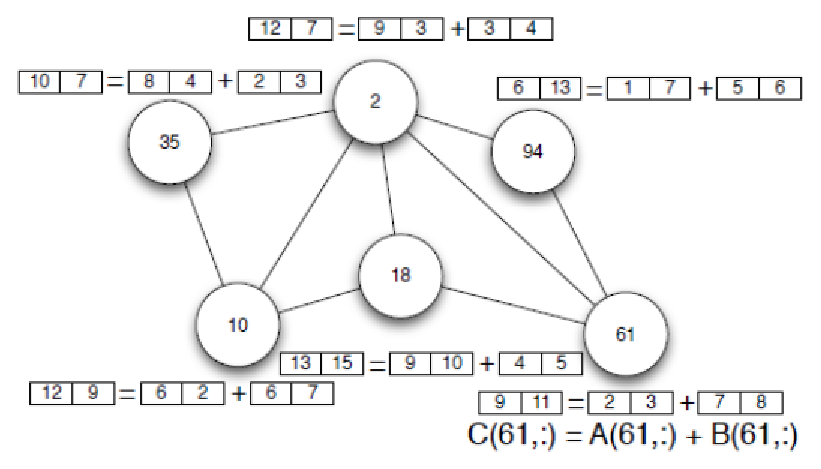
\includegraphics[width=0.8\columnwidth]{fig/DistributedArray.eps}
  \caption[Distributed Macrovector]{Distributed Macrovector: Nodes can read and write their own values in
  the vector.}
  \label{fig:distributedVector}
\end{figure}

\begin{figure}
  \centering
  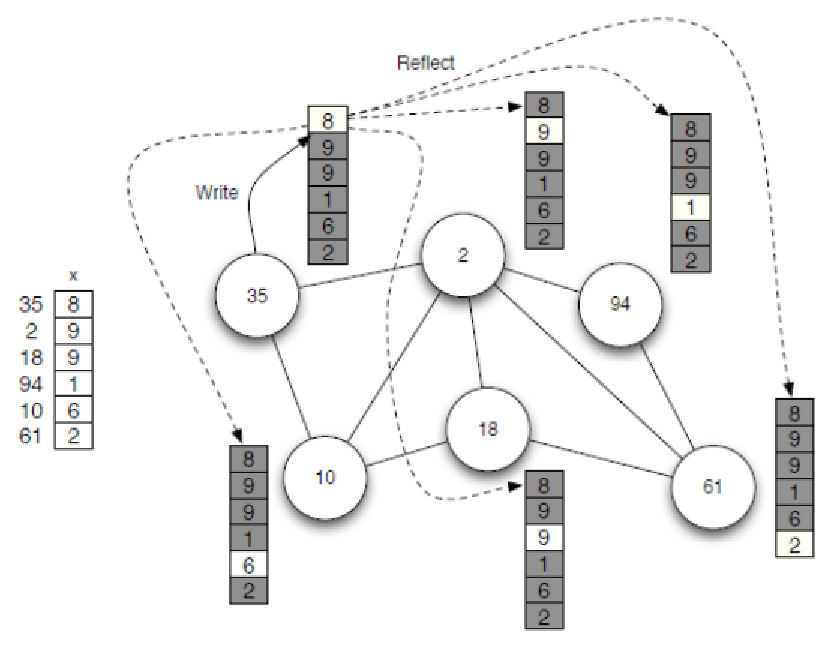
\includegraphics[width=0.8\columnwidth]{fig/ReflectedArray.eps}
  \caption[Reflected Macrovector]{Reflected Macrovector: Nodes can read all values in the vector, but can only write to their own value.}
  \label{fig:reflectedVector}
\end{figure}

{\bf Distributed Representation:} The first way to represent a macrovector is to
store each row on its associated node.  Figure~\ref{fig:distributedVector} shows
how the elements of the macrovectors $A$, $B$, and $C$ from
Figure~\ref{fig:macroVectorAddition} can be stored on each node and how the {\tt
addition} operation is performed. Since elements are only added to corresponding
elements on the same node, this operation can take place without message passing
between nodes.

In general, the distributed representation of macrovectors allows for the
efficient implementation of vector operations that do not span multiple rows.
Conversely, this representation requires significant message passing for
aggregate operations like {\tt max} that require values resident on multiple
nodes. If a macroprogram uses the {\tt max} operation frequently on a particular
macrovector, then a distributed decomposition would be very costly.

{\bf Centralized Representation:} The second representation supported by
MacroLab stores all elements on a single node, typically the base station. This
representation is in diametric opposition to a \emph{distributed}
representation. It allows operations like {\tt max} to be applied with virtually
no explicit message passing cost.  However, there is a potentially significant
cost associated with keeping the elements of the centralized vector
up-to-date. If the values are frequently updated remotely by the sensor nodes,
they need to be frequently transmitted for storage. The centralized
representation is favorable if the vector participates frequently in aggregate
operations that span rows (like {\tt max}). It is less favorable if the vector
is frequently updated with sensor data.

{\bf Reflected Representation:} The third macrovector representation stores all
elements on all nodes. The microcode on each node has read/write access to its
associated element and read-only access to cached versions of all other elements
in the vector. This precludes the need for write-write synchronization since
only one node may write to any given element. However, nodes do need to
communicate their updated values after performing a write, as illustrated in
Figure~\ref{fig:reflectedVector}; when node $35$ writes to its own element in
the vector, the value is {\em reflected} to all other nodes currently caching
it.

This representation is conceptually similar to Reflective Memory (RM), which is
a form of shared memory for parallel systems\cite{Jovanovic}.  It is different
from a neighbor-based macrovector because the scope of a reflected macrovector
is {\em globally defined}; it is not different for each node.  The reflected
representation is beneficial when used by a small {\em group} of nodes that are
relatively close to each other but comparatively far from the base station. In
that situation, the cost of sending information to the base station to perform a
{\tt max} operation is higher than the cost of transmitting to all other nodes
in the group. The reflected representation may also make an operation cheaper
when all nodes need the result.

\subsubsection{Rule-based Microcode Translation}\label{sect:codeTranslation}

Given a representation for each macrovector, the decomposer must produce the
appropriate microcode for each operation in the macroprogram. For example, the
{\tt max} operator must perform different actions when operating over a
distributed vector than when operating over a centralized vector.  To accomplish
this, MacroLab uses a library of microcode templates for each operator and the
different representations of its input parameters.  Thus, {\tt max} would
require three implementations and a binary operator would require $3 \times 3$
implementations. This approach of using a library of operator implementations to
deal with different matrix representations has been used before~\cite{Chang} and
most of this complexity is hidden from the user.

\begin{table}[!htb]
\begin{tabular}{|l|l|l|}
\noalign{\hrule} 
 & & \multicolumn{1}{c|}{$\mathbf{lhs = M(a_1,\ldots,a_n) \ \% \ Synchronous\ Read }$ } \\
\noalign{\hrule}
\multirow{2}{*}{\begin{sideways}Cnt. or Ref.\end{sideways}} & R& %
\tt\begin{tabular}{l} %
owner\_id = RTS.owner(cur\_pc(), M); \\
RTS.notify(cur\_pc(), owner\_id); \\
\end{tabular} \\ \cline{2-3}
 & L & %
% Centralized, local (i.e. MacroLab has control)
\tt\begin{tabular}{l} %
node\_ids = source\_nodes(a1); \\
RTS.wait(cur\_pc(), node\_ids); \\
lhs = local( M(a1,...,an) ); \\
\end{tabular} \\ \noalign{\hrule}
\multirow{2}{*}{\begin{sideways}Distributed\end{sideways}} & R & %
\tt\begin{tabular}{l} %
if (a1 contains node\_id()) then \\
~~owner\_id = RTS.owner(cur\_pc(), M); \\
~~RTS.send(owner\_id, \\
~~~~local(M(node\_id(), a2,...,an) )) \\
~~RTS.notify(cur\_pc(), owner\_id); \\
fi; \\
\end{tabular} \\ \cline{2-3}
 & L &  %
\tt\begin{tabular}{l}%
node\_ids = source\_nodes(a1); \\
RTS.wait(cur\_pc(), node\_ids); \\
lhs = local( M(a1,...,an) ); 
\end{tabular}   \\
\noalign{\hrule}
\end{tabular}
\caption[Pseudocode for mote-level microcode translation of synchronous read] {For each data representation, the row
marked L (for \emph{local}) denotes the code for the mote that will
perform the operation (i.e., the locus of synchronization); R (for
\emph{remote}) marks the code for all other nodes. {\tt M} is a
macrovector; {\tt lhs} and {\tt rhs} are normal vectors. The
mote-local representation of {\tt x} is given by {\tt local(x)}. The
{\tt owner(PC,M)} function gives the ID of the node requesting
the read or write operations on macrovector {\tt M} at
location {\tt PC} in the macroprogram.}
\label{table:synchronousRead}
\end{table}

An implementation of a vector operation will typically consist of multiple
functions, each of which is loaded onto the domain of one of the input
parameters. Tables~\ref{table:synchronousRead} and~\ref{table:synchronousWrite}
shows the various implementations of two basic macrovector operations: reading
and writing one or more elements in a vector. In this context, the vectors {\tt
lhs} and {\tt rhs} are normal vectors and {\tt M} is an n-dimensional
macrovector that is being accessed by indices {\tt a1} through {\tt an}.  These
indices are themselves vectors and index an entire dimension of the matrix {\tt
M}.  The microcode for these operations is different for each of the three
representations discussed in \ref{sect:decompositionTypes}: centralized,
reflected, and distributed.  For each representation, the operation is divided
into two functions: one for the L (\emph{local}) nodes and one piece of code for
the R (\emph{remote}) nodes.

\begin{table}[h]
\begin{tabular}{|l|l|l|}
\noalign{\hrule} 
 & & \multicolumn{1}{c|}{$\mathbf{M(a_1,\ldots,a_n) = rhs \ \% \ Synchronous\ Write}$ } \\
\noalign{\hrule}
\multirow{2}{*}{\begin{sideways}Centralized\end{sideways}} & R& %
\tt\begin{tabular}{l} %
if (a1 contains node\_id()) then\\
~~owner\_id = RTS.owner(cur\_pc(), M); \\
~~RTS.wait(cur\_pc(), owner\_id); \\
fi; \\
\end{tabular} \\ \cline{2-3}
 & L & %
\tt\begin{tabular}{l} %
node\_ids = source\_nodes(a1); \\
local( M(a1,...,an) ) = rhs; \\
RTS.notify(cur\_pc(), node\_ids); \\
\end{tabular} \\ \noalign{\hrule}
\multirow{2}{*}{\begin{sideways}Reflected\end{sideways}} & R & %
\tt\begin{tabular}{l} %
if (a1 contains node\_id()) then \\
~~owner\_id = owner(cur\_pc(), M); \\
~~RTS.receive(owner\_id, \\
~~~~local( M(a1,...,an) )); \\
~~RTS.wait(cur\_pc(), owner\_id); \\
fi; \\
\end{tabular} \\ \cline{2-3}
 & L & %
\tt\begin{tabular}{l} %
node\_ids = source\_nodes(a1); \\
local( M(a1,...,an) ) = rhs; \\
foreach (node\_id in node\_ids) do \\
~~RTS.send(node\_id, \\
~~~~~~~~~~~local( M(a1,...,an) )); \\
done; \\
RTS.notify(cur\_pc(), node\_ids); \\
\end{tabular} \\ \noalign{\hrule}
\multirow{2}{*}{\begin{sideways}Distributed\end{sideways}} & R & %
\tt\begin{tabular}{l} %
if (a1 contains node\_id()) then \\
~~owner\_id = RTS.owner(cur\_pc(), M); \\
~~RTS.receive(owner\_id, \\
~~~~local(M(node\_id(), a2,...,an))); \\
~~RTS.wait(cur\_pc(), owner\_id); \\
fi; \\
\end{tabular} \\ \cline{2-3}
 & L &  %
\tt\begin{tabular}{l}%
node\_ids = source\_nodes(a1); \\
local( M(a1,...,an) ) = rhs; \\
foreach (node\_id in node\_ids) do \\
~~RTS.send(node\_id,\\
~~~~~~~~~~~local( M(a1,...,an) )); \\
done; \\
RTS.notify(cur\_pc(), node\_ids); \\
\end{tabular}   \\
\noalign{\hrule}
\end{tabular}
\caption[Pseudocode for mote-level microcode translation of synchronous write] {For each data representation, the row
marked L (for \emph{local}) denotes the code for the mote that will
perform the operation (i.e., the locus of synchronization); R (for
\emph{remote}) marks the code for all other nodes. {\tt M} is a
macrovector; {\tt lhs} and {\tt rhs} are normal vectors. The
mote-local representation of {\tt x} is given by {\tt local(x)}. The
{\tt owner(PC,M)} function gives the ID of the node requesting
the read or write operations on macrovector {\tt M} at
location {\tt PC} in the macroprogram.}
\label{table:synchronousWrite}
\end{table}

For illustrative purposes, the microcode for the synchronous {\tt read}
(Table~\ref{table:synchronousRead}) and {\tt write}
(Table~\ref{table:synchronousWrite}) operations are shown. The are based on the
standard {\tt notify} and {\tt wait} primitives instead of using message passing
primitives.  {\tt RTS.wait(PC, node\_ids)} causes the current node to block
until each of the nodes in {\tt node\_ids} has called {\tt RTS.notify} with a
matching value for PC. A call to {\tt RTS.notify(PC, node\_ids)} signifies that
the caller has ``caught up'' to a particular program point in the
macroprogram. {\tt RTS.notify} blocks until the corresponding {\tt
RTS.wait}. This is done to prevent the notifying node from overwriting data
before it can be used by the waiting thread.  {\tt RTS.owner} takes the current
location in the macroprogram ({\tt cur\_pc()}) and returns the node ID of the
local node. This ID may be fixed at compile time. Operations over a centralized
macrovector are always performed on the node that has the local copy of that
macrovector. In other cases, such as neighborhood-based operations, the ID of
the local node is unknown until runtime and may change over time.

In principle, this implementation of synchronous {\tt read} and {\tt write}
could be used to implement most macrovector
operations. Figure~\ref{table:maxAndFind} show implementations of synchronous
{\tt max} and {\tt find} functions. The synchronous {\tt max} operation works by
reading {\tt A} into a local variable (which is a normal vector), performing the
operation, and then writing the results.  Thus, this implementation caches the
entire macrovector on a centralized node before performing the operation.  The
code for synchronous {\tt find} assumes the existence of a temporary vector {\tt
Temp} created by the translator to store the result of the find in single-column
form.  Both operations are synchronized because the initial read is
synchronized, although this na\"{i}ve approach incurs a round-trip message
between the local node and each remote node.

\begin{table}[!htb]
\begin{tabular}{l|ll}
{\begin{macrolab}
% smax(A)
sread(A, lvar);
lmax = max(lvar);
write(A, lmax);
.
\end{macrolab}}
& ~ &
{\begin{macrolab}
% sfind(A(1) = 5) 
sread(A, lvar); 
lres =
  find(lvar(1) = 5); 
write(Temp, lres);
\end{macrolab}}
\end{tabular}
\caption{Local half of na\"{i}ve implementations of the synchronous {\tt max} and
{\tt find} functions.}
\label{table:maxAndFind}
\end{table}

In practice, many macro-operations will require specialized
implementations to further reduce messaging overhead.  For example,
the {\tt max} operation could be performed using in-network
aggregation such as that used in Tiny AGgregation
(TAG)~\cite{Madden2002}.  This implementation is a {\em
  semantics-preserving} optimization. It is computationally equivalent
to the na\"{i}ve implementation shown above, but would result in lower
messaging overhead. The following section discuss
optimizations to reduce messaging overhead that are not
semantics-preserving.

\subsubsection{Reducing Synchronization Overhead}

Synchronization is one of the main costs of a MacroLab program; nodes
must send messages to indicate that they have ``caught up'' to a point
in the macroprogram, even if they have no useful data to provide.
This messaging overhead is necessary to preserve the semantics of the
original macroprogram, but many CPS applications do not need strict
synchronization for proper operation.  Consider the example below,
where the intent of this code is to provide a frequently updated
maximum light value.

\begin{macrolab}
every(1000) {
  light = sense(lightSensors);
  maxLight = max(light);
}
\end{macrolab}

\noindent In this case, synchronizing line 3 is unnecessary since the user is
probably not explicitly interested in having {\tt maxLight} represent the
maximum for a particular loop iteration.  Similarly, the synchronized version of
the operation {\tt find(light > 100)} would require a round trip message from
all nodes, including those that have {\tt light} values less than $100$.  An
unsynchronized implementation could require messages only from those nodes that
have values greater than $100$.  These optimizations improve parallelism and
reduce messaging overhead, but do not preserve the original semantics of the
vector operations.  To allow users to employ these optimizations, MacroLab must
provide both synchronized and unsynchronized versions of each operation. The
synchronized versions take function names that start with an \emph{s}: {\tt
smax}, {\tt swrite}, {\tt splus}, etc. The usual notations (e.g., {\tt A + B},
{\tt max(A)}) will refer to the \emph{un}synchronized version of that operation.

It is important to note that not all vector operations require
synchronization.  Operations over macrovectors generally fall into two
categories: {\em row-parallel} operations and {\em inter-row}
operations.  An inter-row operation is any expression that ``mixes''
macrovector domains. For example, an expression like {\tt max(A)}
returns a single-valued result by combining information from all rows
of {\tt A}. Inter-row operations require synchronization to be
semantics-preserving, but alternative implementations with different
semantics can be used in order to reduce overhead.  Conversely, a
statement like {\tt A = A + B} is {\em row-parallel}: the operation
over any particular row does not require information from any other
row, and so the operation can be performed over each row without
waiting for A and B to be fully updated.  When multiple row-parallel
operations occur consecutively, their execution may overlap.

Generally, inter-row operations are more expensive than row-parallel
operations because of the synchronization required.  The difference
between row-parallel and inter-row operations is evident from the
source code, providing the user with a {\em clear cost model} of the
macroprogram and empowering the user to write optimized code
that will produce efficient decompositions.  Furthermore, the
user can control the amount of synchronization overhead by
choosing between synchronized and unsynchronized versions of each
inter-row operation.

\subsection{Cost Analyzer} \label{sect:costAnalyzer}

\begin{figure}[ht]
  \centering
  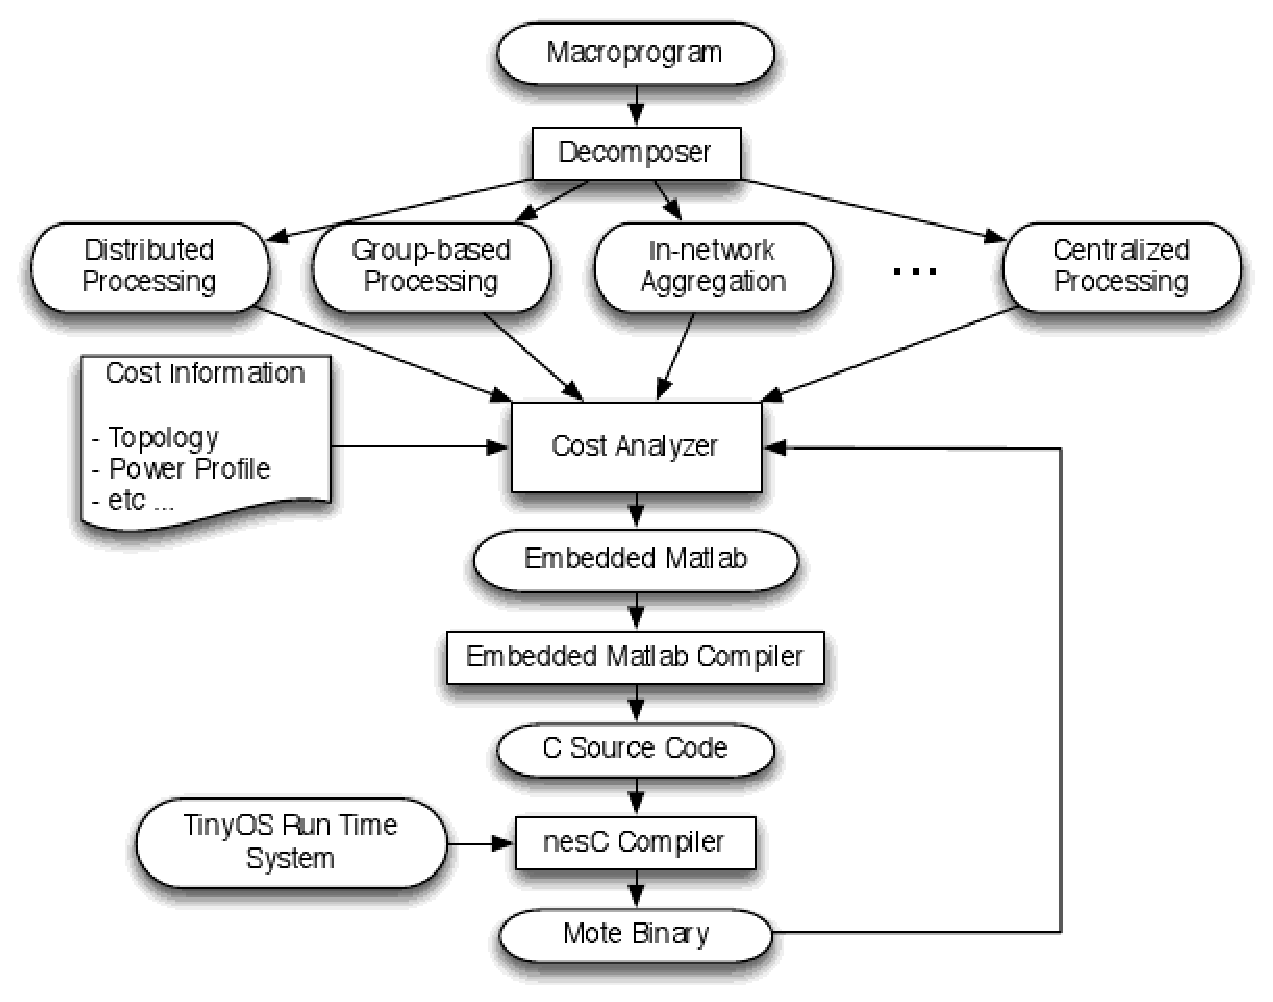
\includegraphics[width=0.8\columnwidth]{fig/System.eps}
  \caption[MacroLab system architecture]{MacroLab consists of a decomposer, a
  cost analyzer, and a run-time system. In this implementation, all possible
  decompositions of a macroprogram are generated and then analyzed and compare
  them based on the cost profile of a target deployment.}
  \label{fig:System}
\end{figure}

The decomposition process produces many feasible candidate program
decompositions. The goal of cost analysis is to predict which
candidate will be most efficient for a target deployment.  Two
different techniques for cost analysis are used: compile-time analysis and
run-time analysis.  As shown in Figure~\ref{fig:System}, an initial
decomposition might be chosen using the static analysis until richer
run-time profile information is available. Cost analyses can be based
on a number of different cost functions such as power, bandwidth,
messages, or latency.  In this dissertation, only messaging cost is considered.

\subsubsection{Static Cost Analysis}\label{sect:staticCost}

The static analysis approximates the true messaging cost of a MacroLab
program based on (1) user-provided cost information for messages, (2) sensing event
frequencies, (3) a description of the deployment network, and (4) a conservative
analysis of the source code to locate network sends. The cost information
is provided as a matrix indicating hop counts between nodes. The high-level
structure of the static cost anlayzer is as follows: 

\begin{macrolab} 
totalCost = 0; 
foreach node x in the network do 
  cost[x] = 0;
  foreach predicted send in one run of x do
    cost[x] += hop_count[x,target_of_send] * frequency_of_this_event_at_this_node;
  done;
  totalCost += cost[x];
done;
return totalCost;
\end{macrolab} 

It is assumed that the MacroLab program follows a main event-loop format (as in
lines 4--7 of Figure~\ref{code:Surge}, lines 6--12 of Figure~\ref{code:PEG}, or
lines 10--17 of Figure~\ref{code:BusTracking}) and predict the cost for one run
through that loop. An intraprocedural dataflow analysis is used to scan the
statements in the program's main loop for predicted sends (line 4).

Each statement that contains a macrovector operation, such as a read from a
sensor array, is considered. Based on the decomposition, the operation is
analyzed to determine if it involves remote or distributed operations and thus,
message sends. If the destination of the message cannot be statically
determined, the maximal hop cost from the current node, which is a conservative
estimate, is used. The hop cost is weighted by the relative frequency of that
event.

Note that it is not possible for a distributed operation to trigger
other distributed operations in MacroLab; the user cannot write
messaging code directly and all sends and receives are inserted by the
decomposer and mediated by the run-time system. There are no message
loops to consider and it suffices to consider each node separately to
calculate a total predicted cost. 

If the user does not have a model of the sensing event frequencies at each
node, the analysis assumes events will occur with equal frequency across
all nodes for all decompositions. A final cost estimate can be
produced that is relative to the number of sensing events. In such a
scenario, the cost analyzer does not predict the actual messaging cost of a
decomposition but still provides a useful heuristic for distinguishing
\emph{between} two candidate decompositions.  

Note that a more precise dataflow analysis for predicting statement frequencies
(e.g.,~\cite{Ramalingam}) could be used. However, the message costs would still
have to be modeled, the network topology understood, and the event frequencies
predicted.  In the experiments presented in this dissertation these were the
determining factors and the MacroLab programs themselves were small and easy to
analyze.


\subsubsection{Run-time Cost Analysis}\label{sect:runtimeCost}

A run-time analysis to measure the costs of a deployed decomposition can also be
performed. The decomposer is used to inject logging code at appropriate
locations in the microprogram to count the messages that are actually being
sent. Logging code can also be injected to estimate how many messages {\em would
be} sent by other decompositions (as in Tables~\ref{table:synchronousRead}
and~\ref{table:synchronousWrite}). The logged information is periodically
analyzed by the cost analyzer to ensure that an efficient version of the
implementation is executing. If the currently-executing version is more costly
than an alternative, the network can be reprogrammed with the alternative
decomposition. Currently, it is not possible to reprogram the network without
losing the state of the program that was generated by a different decomposition,
but this will be analyzed in future work.


\subsection{Compilation and Run-Time System} \label{sect:RTS}

The run-time system supports three operations for \\MacroLab
microprograms: (1) networking, (2) hardware access, and (3) accessor
functions to information such as node ID, current time, location,
radio neighbors, etc.  The RTS is written as a nesC module and supports
the functions shown in Table \ref{table:lib}.  The first three
functions are provided directly by the RTS while the
last three functions must interface with TinyOS libraries for capabilities
such as time synchronization and networking operations.  By interfacing
with TinyOS, MacroLab leverages an existing suite of distributed
algorithms as well as ongoing advances and future software
development.  

\begin{table}[!htb]
  \centering
   \begin{tabular}{| l |}
     \hline
     \multicolumn{1}{|c|}{Operation} \\
     \hline
     getID() \\
     \textit{returns the node's ID}\\
     \hline
     getProperty('property') \\
     \textit{returns a generic property of a node} \\
     \hline
     getNodes('group') \\
     \textit{returns the current membership in a global group}\\
     \hline
     getTime() \\
     \textit{returns the current global time} \\
     \hline
     getNeighbors() \\
     \textit{returns the current radio neighbors of a node}\\
     \hline
     remoteFeval(nodeIDs,funcName,\{P1,P2,...,Pn\}) \\
     \textit{remote function invocation}\\
     \hline
   \end{tabular}
   \caption[Functions supported by the Run-Time System]{The RTS must provide an interface for
   neighbor discovery, time sync, and remote function calls.}
   \label{table:lib}
\end{table}

The {\tt remoteFeval} function is a generic messaging interface
provided to the MacroLab microprograms.  It is similar to Matlab's
{\tt feval} function in that it takes a function handle and a set of
arguments and invokes that function with those arguments.  However,
{\tt remoteFeval} invokes the function on a set of remote nodes
indicated by the {\tt nodeIDs} parameter.  The function name and
arguments are marshalled into a packet, sent to those nodes, and
unmarshalled before the function is invoked.  The {\tt remoteFeval}
function can take an arbitrary set of nodeIDs and the RTS decides the
best way to send the message.  For example, if nodeIDs only contains
the ID of the base station node, the RTS sends the message using a
standard TinyOS routing protocol.  If nodeIDs only contains IDs of
neighboring nodes, the RTS sends the message using a local broadcast.
In the current implementation, the RTS will flood the message to all
nodes for any other set of nodeIDs, but multi-cast algorithms or other
routing algorithms could easily be inserted as they are developed.  

Access to hardware such as sensors and actuators must be done through new
functions provided by user defined hardware drivers.  The {\tt BASE\_DISPLAY}
and {\tt CAMERAFOCUS} functions shown in Figures~\ref{code:Surge}
and~\ref{code:PEG} would simply be C functions provided by the user that would
set the input/output pins of the microcontroller based on the input parameters.
In the case of split-phase functions like {\tt sense}, the driver must declare
the name of the callback that will be triggered when the function is complete.
The decomposer then generates the appropriate code using this callback to
continue execution in the microprogram.  The actual light sensor driver used by
the code in Figure~\ref{code:Surge} is shown in Figure~\ref{code:hardwareDriver}.

\begin{figure}[h]
  \begin{nesc}
module LightSensorP {
  provides interface LightSensor;
  uses interface Read<uint16_t> as Read;
}
implementation
{
  command void LightSensor.sense() {
    call Read.read();
  }
  event void Read.readDone(error_t err,
   uint16_t val) {
    if(err == SUCCESS) {
      #CALLBACK(val);
    }
  }
}
  \end{nesc}
  \caption[A split-phase hardware driver for reading from the light sensor]{The
  {\tt LightSensor.sense} function is called by the microcode through the RTS.
  The decomposer must automatically replace {\tt\#CALLBACK} with an appropriate
  function to continue microprogram execution.}
  \label{code:hardwareDriver}
\end{figure}

In order to conserve power, MacroLab enables the TinyOS 2.x low-power listening
capabilities~\cite{Polastrea}, which automatically duty cycles the radio and
sends messages with long preambles.  The RTS dynamically sets the sleep interval
of the radio based on the number of messages currently being sent by the
application.  The entire network starts with a default sleep interval of 100
milliseconds and nodes will flood the network to halve or double the sleep
interval when total transmission time is greater than 80 percent or less than 20
percent.  Thus, the radio sleep interval for the entire network is dynamically
set based on the node with the highest load.  This simple algorithm will not
always be optimal, but it works well for the existing applications, as shown in
Section~\ref{sec:performance}, more sophisticated adaptive algorithms will be
explored in future work.  MacroLab programs are executed on
Telos~\cite{Polastre} nodes, for which the TinyOS libraries automatically use
low-power mode when idle.

The MacroLab microprogram, the RTS, and the TinyOS libraries are compiled
together into a single binary executable (Figure~\ref{fig:System}) that can run
on mote-class devices such as the MICA~\cite{Crossbow} and the Telos.  The
microprogram generated by the decomposer is written in Embedded Matlab, a
simplified form of the Matlab syntax that does not support dynamic typing or
dynamic memory allocation.  This is compiled down to C code by the Embedded
Matlab compiler, provided by The MathWorks~\cite{mathworks}.  This C code is
then compiled together with the nesC RTS module and the TinyOS libraries by the
nesC compiler.

\section{Evaluation} \label{sect:evaluation}

MacroLab is evaluated in four parts. First, the programming abstraction is
evaluated by showing that it is expressive enough to implement canonical CPS
applications, such as data collection and object tracking. Second, the overhead
of running MacroLab programs is compared with similar programs written using
nesC and TinyOS. Third, a MacroLab application is deployed in multiple different
scenarios and measure the effect of DSCD on message cost. Finally, the accuracy
of the static cost analyzer is evaluated.

\subsection{Expressiveness of the Abstraction}\label{sect:expressiveness}

The expressive power of the programming abstraction is evaluated by showing that
it can be used concisely to implement two canonical CPS applications: {\em
tree-based data collection} in Surge~\cite{Gay} and {\em object tracking} in the
Pursuer-Evader Game (PEG)~\cite{Sharp}. These two applications were selected
because they represent basic algorithms that have been incorporated into many
other CPS applications.  Table~\ref{table:LOC} presents a comparison of the
number of lines of code necessary to implement Surge and PEG in MacroLab as
compared to their original implementations in nesC/TinyOS. The number of lines
of code for the nesC/TinyOS implementations of Surge and PEG were cited from
previous publications~\cite{Muller,Kothari}.  The MacroLab applications are
about one-fiftieth the size of equivalent nesC/TinyOS implementation in terms of
lines of code. This ratio is typical of the difference in size between
equivalent Matlab and C programs. MacroLab builds a considerable amount of logic
such as routing algorithms and vector operations into the run-time
system. MacroLab dramatically reduces the amount of code and therefore the
amount of development and maintenance time required to implement basic CPS
applications.

The MacroLab programming abstraction is suitable for many application domains,
but it cannot express algorithms that require explicit message passing. For
example, it cannot easily be used to implement routing protocols, time
synchronization protocols, or other distributed middleware libraries.  Instead,
all of these operations must be incorporated into the run-time system. Thus,
MacroLab programs are limited to distributed operations that can be neatly
stored in a library and provided by some interface. This it not a restricting
requirement for most CPS software. However, it can make it difficult to provide
application-specific distributed operations. Developers must encapsulate such
functionality by extending the run-time system. Code movement in systems like
Agilla~\cite{Fok} and EnviroSuite~\cite{Luo} might be difficult to implement in
MacroLab.

\begin{table}[!htb]
\centering
\begin{minipage}{\columnwidth}
\centering
\begin{tabular}{|c|c|c|}
\cline{2-3}
\multicolumn{1}{c|}{}&MacroLab&nesC/TinyOS\\
\hline
Surge&7&400\\
\hline
PEG&12&780\\
\hline
\end{tabular}
\end{minipage}
\caption[Lines of code (LOC) comparison]{Comparison of lines of code required for equivalent
functionality in two basic CPS applications.}
\label{table:LOC}
\end{table}

\subsubsection{Surge}\label{sect:surge}

Surge is a simple application that periodically collects sensor readings from
all nodes and routes them back to a base station.  The data collection aspect of
Surge has been widely utilized in many sensor network applications. In fact,
many sensor network applications, such as~\cite{Mainwaring,Juang,Selavo},
involve primarily data collection and in many other applications, such as
AlarmNet~\cite{Wood}, data collection plays an important role. Thus, it is
essential that an abstraction for sensor network programming make it easy to
implement data collection applications.  Figure~\ref{code:Surge} shows the
source code for Surge written in MacroLab.  In line~1, the run-time system is
instantiated and in lines~2 and~3, it is used to instantiate a vector of light
sensors (one for each node in the network) and a macrovector to hold the light
values.  Line~4 is the beginning of a loop that occurs every 1000 milliseconds.
The light sensors are read in line 5 and the values are displayed at the base
station in line 6.

\begin{figure}[h]
  \begin{macrolab}
RTS = RunTimeSystem();
lSensors = SensorVector('lightSensor','uint16');
lightValues = Macrovector('uint16');
every(1000)
  lightValues =  sense(lSensors);
  BASE_DISPLAY(lightValues);
end
  \end{macrolab}
  \caption[A data collection application (Surge) in MacroLab]{Surge reads sensor
  values and displays them at the base station.  {\tt BASE\_DISPLAY} is
  implemented within the RTS and sends a message to a base station for display.}
  \label{code:Surge}
\end{figure}

There is hidden complexity in the interaction between lines 5 and 6. The
decomposer identifies that the sensor resources are on the nodes while
the {\tt BASE\_DISPLAY} function is only available on the base station.  It
therefore infers that the information created in line 5 must be routed
across machine boundaries in order to be used in line 6 and the
compiled version of the code automatically invokes the routing algorithm
via the {\tt remoteFeval} interface described in Section~\ref{sect:RTS}.
The high-level algorithm can be expressed in seven lines of MacroLab. 
The automatically generated microcode that runs on the nodes is closer
in size to the nesC/TinyOS implementation. 

\subsubsection{Pursuer-Evader Game (PEG)}\label{sect:peg}

\begin{figure}[ht]  
  \begin{macrolab}
motes = RTS.getMotes('type', 'tmote')
magSensors = SensorVector(motes, 'magnetometer');
magVals = Macrovector(motes);
neighborMag = neighborReflection(motes, magVals);
THRESH = uint8(500);
every(1000)
  magVals =  magSensors.sense();
  active = find(sum(neighborMag > THRESH, 2) > 3);
  maxNeighbor = max(neighborMag, 2);
  leaders = find(maxNeighbor(active) == magVal(active));
  CAMERAFOCUS(leaders);
end
  \end{macrolab}
  \caption[A tracking application (PEG) in MacroLab]{Every 1000\ms, nodes take a
  reading from their magnetometers and share the values with their neighbors.
  If more than three nodes in a neighborhood sense a magnetometer value about a
  threshold, a leader is elected from among them and a camera is focused on
  it. {\tt CAMERAFOCUS} is implemented within the RTS and sends a message to the
  camera, which is at the base station.}
  \label{code:PEG}
\end{figure}

The Pursuer-Evader Game (PEG) is a distributed CPS application that detects and
reports the position of a moving object within a sensor field.  It is a
canonical application in the field of robotics research where multiple robots
(the pursuers) collectively determine the locations of one or more evaders and
attempt to corral them. This application has been adapted by the sensor network
community~\cite{Sharp,Brooks,Li} and represents the algorithmic capabilities
necessary for a number of canonical applications such as object tracking and
in-network filtering of false positives. It is widely used as an application for
the evaluation of sensor network programming abstractions and
architectures~\cite{Whitehousea,Kothari,Gnawali} since it is one of the largest
TinyOS applications and utilizes a number of relatively sophisticated concepts
for sensor networks.  Figure~\ref{code:PEG} shows an implementation of PEG in
MacroLab in which the network routes the location of the evader to a camera
which visually follows the evader. In lines~1--3 the code initializes the {\tt
motes} vector of node IDs, the {\tt magSensors} vector of magnetometer sensors,
and the {\tt magVals} macrovector of magnetometer readings.  In line 4, a $n \
\times \ n$ {\tt neighborReflection} macrovector is created where each element
$i,j$ has a cached copy of the $j$th element of {\tt magVals} if $i$ is a
neighbor of $j$, and an invalid value otherwise.  In the main loop, every
1000\ms, line 7 reads from all magnetometer values and line~8 creates an
{\tt active} vector with the IDs of all nodes that have at least three neighbors
with values higher than {\tt THRESH}. Since {\tt sum} returns the sum over
columns by default, the second parameter, 2, to {\tt sum} indicates the sum
across rows to be calculated since each row contains a particular node's
neighborhood. Line~9 creates a {\tt maxNeighbor} vector with the highest
sensor value in each node's neighborhood. Here too the 2 as the second parameter
indicates that the maximum value across nodes should be calculated instead of
across columns. Line~10 creates a {\tt leaders} vector, which contains the IDs of
those nodes that have the highest sensor value in an active
neighborhood. Finally, line~11 uses a proprietary function called {\tt
CAMERAFOCUS} to focus all available cameras on the leader nodes, using a
pre-defined mapping from nodeID to location. The user, or camera manufacturer,
would need to write the {\tt CAMERAFOCUS} function, which is basically a
hardware driver, while the standard Matlab functions such as {\tt find}, {\tt
sum}, and {\tt max} are provided by the MacroLab system. The hardware drivers
for the sensors are also provided by the MacroLab system by using the TinyOS
operating system.  The purpose of this example is to demonstrate that MacroLab
can concisely represent efficient, neighborhood-based, in-network processing.


\subsection{Performance Overhead} \label{sec:performance}

To evaluate the performance overhead of MacroLab, the resource consumption of
the two applications described in Section~\ref{sect:expressiveness} is measured
and compared against existing applications written in nesC/TinyOS. MacroLab
programs are very similar to TinyOS programs in terms of memory footprint,
execution speed, and power consumption.

The program size and heap size of two MacroLab programs is shown in
Table~\ref{table:CodeSize}, along with those of several existing TinyOS
programs.  The MacroLab programs actually have a smaller memory footprint than
their corresponding TinyOS implementations, both in terms of program memory and
RAM. While the TinyOS versions may be somewhat more feature rich, the MacroLab
versions are still not much larger than extremely simple TinyOS applications
such as {\tt SenseToRfm}.  Table \ref{table:CodeBreakdown} shows the breakdown
of the MacroLab programs' memory footprints.  This information was collected by
examining the symbol table of the final binary executables.  Therefore any
variables or code removed by compiler optimizations are not included. The vast
majority of the program size of MacroLab applications (approximately 17KB of ROM
and 600 bytes of RAM) is due to imported TinyOS libraries for multi-hop routing,
access to the Analog-to-Digital Converter (ADC), and the Timer.  The run-time
system module requires 558 bytes of program memory and 66 bytes of RAM.  For
both PEG and Surge, the application logic itelf required less than 1.3KB of ROM
and 150 bytes of RAM.


\begin{table}[!htb]
  \centering
  \begin{minipage}{\columnwidth}
    \centering
    \begin{tabular}{|l|r|r|}
      \hline
      \multicolumn{1}{|c}{Application} & \multicolumn{1}{|c|}{Program Size} & \multicolumn{1}{c|}{Heap Size}\\
      \hline
      TelosB&49,152&10,240\\
      MICAz&131,072&4,096\\
      \hline
      Blink&2,472&38\\
      CountRadio&11,266&351\\
      Oscilloscope&9,034&335\\
      OscilloscopeRF&14,536&449\\
      SenseToRfm&14,248&403\\
      TOSBase&10,328&1,827\\
      \bf{MacroLab\_Surge}&19,374&669\\
      SurgeTelos&24,790&911\\
      \bf{MacroLab\_PEG}&18,536&770\\
      PEG~\cite{Sharp}&61,440&3,072\\
      \hline
    \end{tabular}
  \end{minipage}
  \caption[MacroLab code size evaluation]{Program and heap size comparison for common TinyOS applications and two
  MacroLab applications for TelosB nodes.}
  \label{table:CodeSize}
\end{table}

The maximum run-time stack sizes of the MacroLab and nesC Surge implementations
are compared. Memory was filled with a special reference pattern, and a program
runf for 600 seconds. Then the high water mark for stack growth was computed by
looking for the last byte not containing the reference pattern.  MacroLab's RTS
layer introduces additional functions and could therefore potentially require
more memory for the stack.  However, aggressive function inlining by the nesC
compiler causes the function call depth to be almost the same for both
applications. The TinyOS version requires 120 bytes while the MacroLab version
requires 124 bytes for the stack, as shown in the last column of
Table~\ref{table:ExecutionTime}.

\begin{table}[!htb]
  \centering
  \begin{minipage}{\columnwidth}
    \centering
    \begin{tabular}{|l|c|c|c|}
      \hline
      \multicolumn{1}{|c}{Application} & \multicolumn{1}{|c|}{TinyOS} & \multicolumn{1}{c|}{RTS} & \multicolumn{1}{c|}{MacroLab}\\
      \hline
      MacroLab\_PEG&16714/579&558/66&1264/125\\
      MacroLab\_Surge&15714/579&558/66&1144/24\\
      \hline
    \end{tabular}
  \end{minipage}
  \caption[MacroLab memory footprint]{A breakdown of the amount of flash/RAM in the TinyOS libraries, RTS,
  and program logic of MacroLab applications}
  \label{table:CodeBreakdown}
\end{table}

To compare the execution speed of a MacroLab program with a TinyOS program, the
time to execute Surge from the beginning of the loop when the node reads the
sensor until the radio has accepted the message for transmission is measured.
These times do not include the Media Access Control (MAC) and transmission
delays.  This time was measured for both the MacroLab and TinyOS implementations
using an oscilloscope.  The first two columns of Table~\ref{table:ExecutionTime}
show that the total execution time was about 18 milliseconds for both programs,
but the MacroLab program takes about 3 percent longer (0.5 milliseconds).  The
CPU was idle for most of the execution, waiting for the ADC to return a value.
The non-idle time for the MacroLab program was 705 microseconds compared with
361 microseconds for the TinyOS program.  Thus, the MacroLab program requires
almost twice as many instructions to be executed as the TinyOS program.  This is
a large multiple, but the effect on overall execution time and power consumption
is small.

\begin{figure}
  \centering
  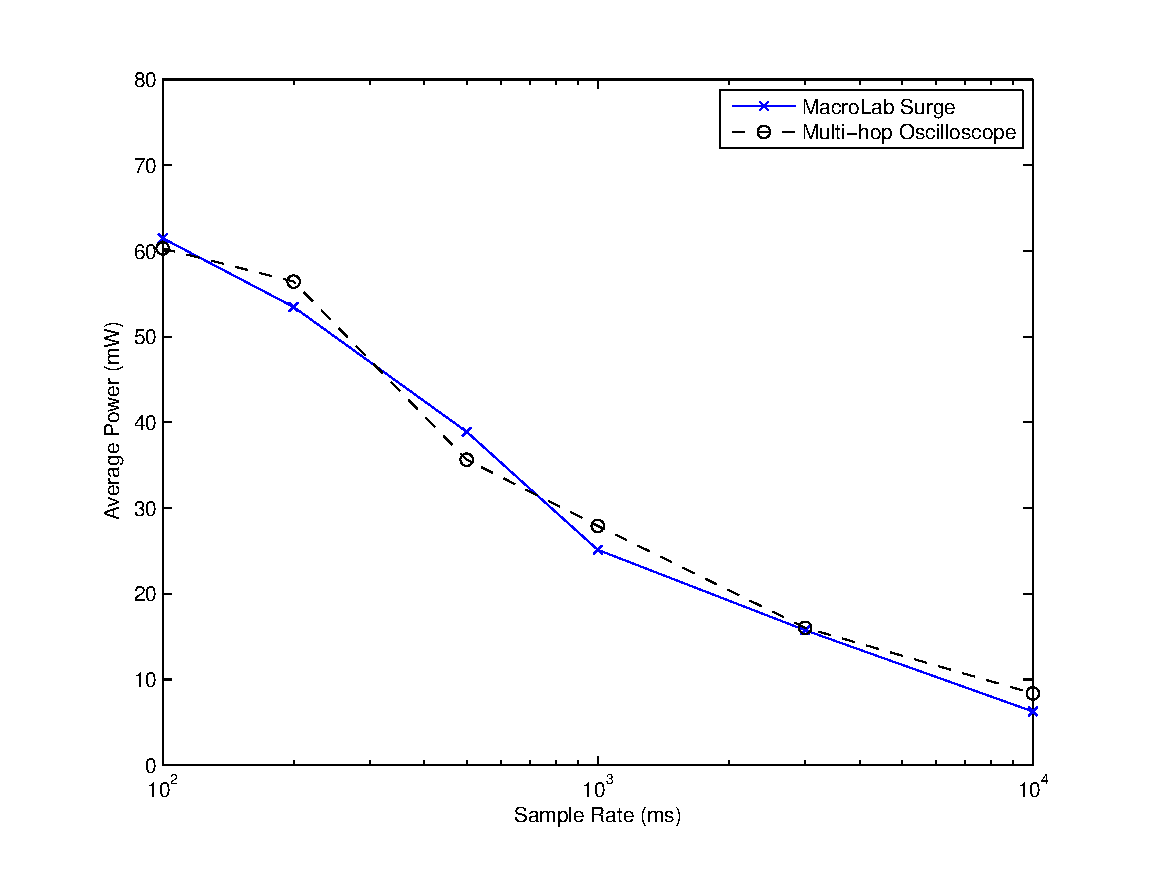
\includegraphics[width=0.6\columnwidth]{fig/SurgePower}
  \caption{Oscilloscope power measurements of MacroLab and nesC Surge
  implementations.} 
  \label{fig:macrolabPowerConsumption}
\end{figure}

The power consumption of both implementations of the Surge application is shown
in Figure~\ref{fig:macrolabPowerConsumption}.  In both cases, power consumption was
measured using an oscilloscope on a node that was forwarding messages from
exactly two children.  The period with which Surge sampled the sensor and
forwarded the message to the base station was varied from 100 milliseconds to 10
seconds. The results show that the average power consumption over a sample run
of 100 seconds is nearly identical for both implementations, even as the
sampling frequency changes by over two orders of magnitude.  This evidence
suggests that MacroLab programs can match TinyOS programs in terms of power
efficiency.

\begin{table}[!htb]
  \centering
  \begin{minipage}{\columnwidth}
    \centering
    \begin{tabular}{|l|r|r|r|}
      \hline
      \multicolumn{1}{|c}{Application}& 
      \multicolumn{1}{|c|}{Execution} &
      \multicolumn{1}{|c|}{CPU} &
      \multicolumn{1}{c|}{Stack}\\
      \hline
      Surge&17.7msec&361usec&120bytes\\
      \bf{MacroLab\_Surge}&18.2msec&705usec&124bytes\\
      \hline
    \end{tabular}
  \end{minipage}
  \caption[Execution time analysis]{An evaluation of the execution time of the application, logic (CPU), and maximum
  consumed stack memory.}
  \label{table:ExecutionTime}
\end{table}


\subsection{Effect of DSCD on Performance}\label{sect:PerformanceEval}

To evaluate the effect of DSCD on the performance of an application in multiple
scenarios, a {\em bus tracking} application (Figure~\ref{code:BusTracking}) was
implemented.  In order to easily modify the deployment scenario, this part of
the evaluation was performed in simulation.  In the bus tracking application,
each bus stop records arrival times for the buses and computes estimated arrival
times for all other buses. The application logic is shown in
Figure~\ref{code:BusTracking}, which maintains state about the last time a bus
was seen at every stop, the time it takes to travel from each stop to every
other stop, and the estimated time that each bus will next arrive at every stop.

\begin{figure*}[ht]
  \begin{macrolab}
    RTS = RunTimeSystem();
    busstops = RTS.getNodes('stopnode'); 
    buses = RTS.getNodes('bus');
    estimates = Macrovector(busstops, length(buses) ,'uint16');
    arrivals = Macrovector(busstops, length(buses) ,'uint16'));
    travelTime = Macrovector(busstops, length(busstops), length(buses) ,'uint16'));
    busSensors = SensorVector('BusSensor',busstops,'uint16');
    routes = uint8({[1 2 3 4], [ 5 6 7 8]}); %Example routes

    while(1)
      [busID,r] =  sense(busSensors);
      busTime = RTS.getTime();
      travelTime(routes{r},routes{r},busID)[1,3] = busTime - arrivals(routes{r}, busID);
      arrivals(routes{r},busID)[1,2] = busTime;
      estimates(routes{r},busID) = travelTime(routes{r},routes{r},busID)[2,3] + busTime;
      BASE_DISPLAY(estimates(routes{r},:));
    end
  \end{macrolab}
  \caption[A bus tracking application in MacroLab]{MacroLab code for the bus
  tracking application.}
  \label{code:BusTracking}
\end{figure*}

First, a bus is sensed at each stop and collect a time stamp of the bus arrival
as {\tt busTime}. The {\em arrivals} matrix stores the last time before now that
each bus arrived at each stop and \textit{travelTime} is updated to be
\textit{busTime} minus \textit{arrivals}. In other words, the travel time
between stops is estimated to be the current time that each bus arrived less the
last time that bus was seen at every other stop. \textit{Arrivals} is then
updated with the current arrival time of the bus. Next, the \textit{estimates}
vector is updated to be \textit{travelTime} plus \textit{busTime}. The predicted
arrival time for each bus is estimated to be its travel time plus the last time
it was seen at all stops. Finally, the estimated arrival times are displayed to
potential passengers using the {\tt BASE\_DISPLAY} operation.  The matrix
operations in this application make heavy use of the dot product notation
described in Section~\ref{sect:dotProduct} for conciseness and efficiency.

MacroLab's row-level parallelism allows the matrix operations to occur
in parallel.  In this particular application, the program runs
correctly without using the synchronized implementation of any
inter-row operations, and so the assignment in line 15 does not block
until all values are collected.  Each row can be processed in parallel
as buses arrive at different stops.

\begin{figure}
  \centering
  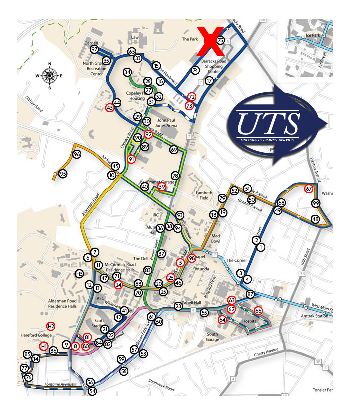
\includegraphics[width=.6\columnwidth]{fig/UTSBusRoutes}
  \caption[University Transit Service (UTS) bus routes at the University of
  Virginia (U.Va.)]{UTS Bus Routes at U.Va. The base station is indicated as a
  cross at the top of the figure.}
  \label{fig:UTS}
\end{figure}

This application is evaluated in four scenarios: 1) the estimated bus arrival
times are displayed to the passengers on a website which is updated from a
centralized base station, 2) the estimated bus arrival times are displayed to
the passengers at each bus stop, 3) the base station radio range is increased
substantially for better coverage, and 4) an additional bus route is added by
the bus company. The results show no decomposition is best for all target
deployments and choosing the correct decomposition can reduce messaging
costs by an average of 44 percent.

MacroLab can optimize for a number of cost metrics (such as latency, power
consumption, or message cost) by using a cost profile and a cost analyzer that
analyzes the cost of each program decomposition for a target deployment
scenario. In this evaluation, only the total number of messages that must be
sent by the network to achieve the global objective is optimized.

\subsubsection{Experimental Setup}\label{sect:setup}
The test scenario consists of actual bus routes at the University of Virginia,
provided by the University Transit Service (UTS), shown in Figure~\ref{fig:UTS}.
It is assumed that each bus stop has a mote and can sense the bus currently at its
stop.  The cost profile of the test scenario was created based on the actual
locations of the bus stops and assuming a reliable communication range of 500 meters

In order to test this wide variety of deployment scenarios, a Matlab-based
simulator was built for this part of the evaluation.  The simulation environment
for MacroLab only requires a slight modification to the RTS in order to support
function calls into the simulator instead of directly to the nodes.  The
simulator runs code similar to microcode that would run on a mote-based RTS.  In
this experiment, only two decompositions are evaluated: a centralized and
distributed decomposition.

Communication between nodes is provided by the RTS. Based on the cost profile
of the network, the simulation observes the total message cost for each
decomposition and scenario.  The cost matrix is computed from the topology
of the scenario and encodes the cost to send messages between pairs of nodes.
The RTS currently supports point-to-point routing but more routing algorithms
can be added as they are developed.

\begin{figure}[t]
  \centering
  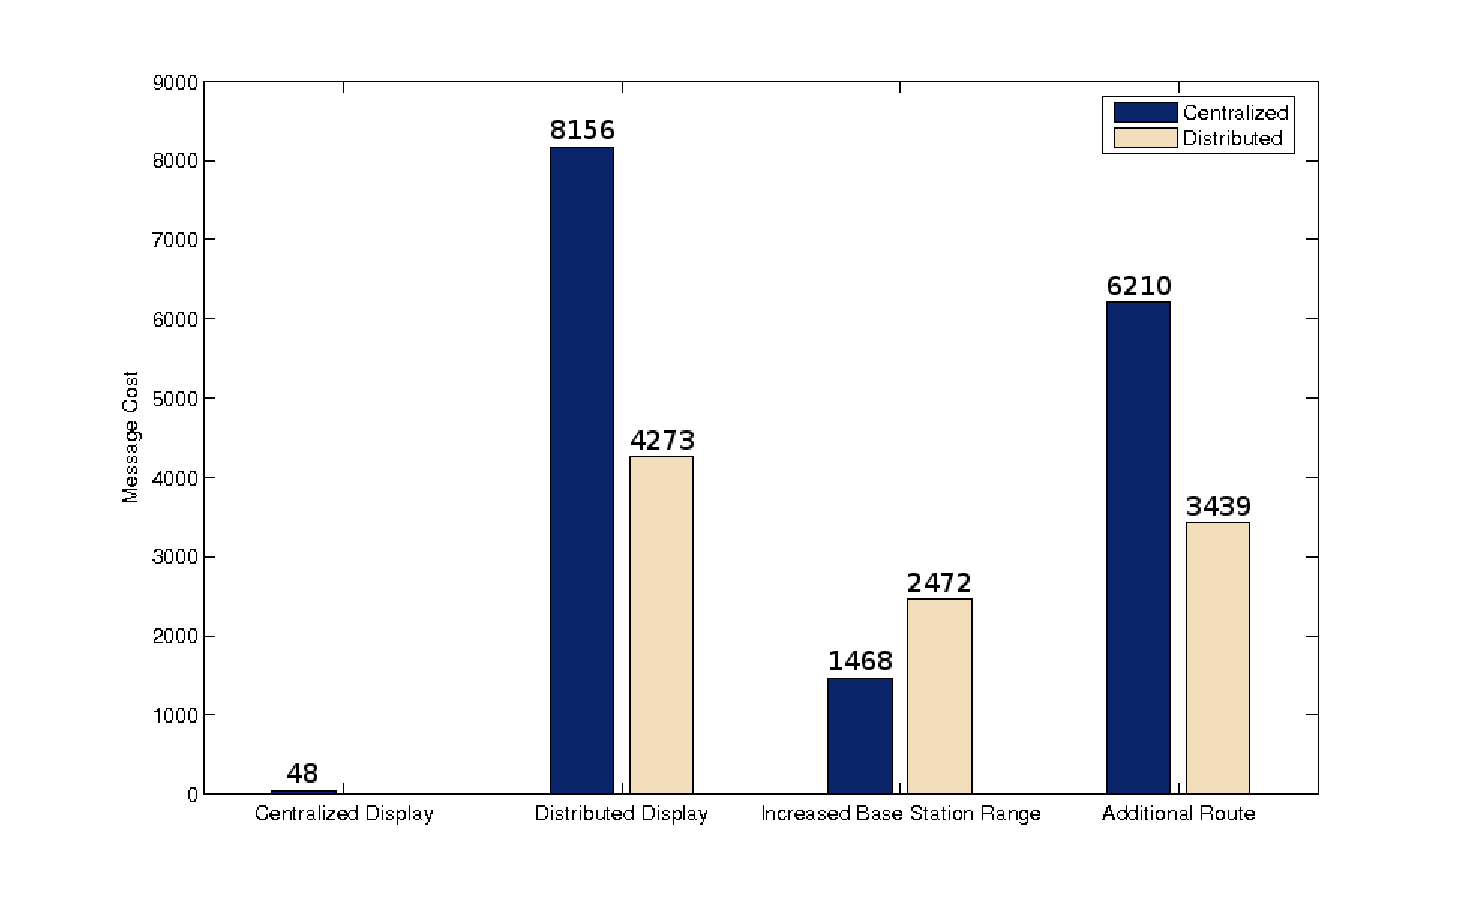
\includegraphics[width=0.8\columnwidth]{fig/scenarioSmall}
  \caption[Effect of deployment scenario on efficient implementation]{Neither
  decomposition is best for all deployment scenarios. Small changes in the
  deployment scenario changes the optimal implementation between centralized and
  distributed.}
  \label{fig:MainResult}
\end{figure}

\subsubsection{Scenario 1: Website Display} 

In the first scenario, the bus information is recorded and displayed on a
website using a centralized base station.  This is accomplished by using the
{\tt BASE\_DISPLAY} operation which can only be executed in a centralized
fashion.  In order to accomplish this version of the application, the nodes will
sense buses and send their data directly back to the base station which will
maintain state in all of the macrovectors and perform all of the vector
computations.  The messaging cost of this application is the same as the Surge
application.  Only one bar is shown in Figure~\ref{fig:MainResult} because the
{\tt BASE\_DISPLAY} operator is only defined for centralized decompositions.  By
running this decomposition in simulation, the cost of running the application
using this scenario is found to be 48 messages over a 30 minute simulation.

\subsubsection{Scenario 2: Bus Stop Displays} 

Changing {\tt BASE\_DISPLAY} to {\tt MOTE\_DISPLAY} allows the application to
show the data at each bus stop rather than at the base station. Sending and
receiving bus arrival information between all nodes within each route totals
8156 messages for the centralized implementation and 4734 for the distributed
version; the distributed decomposition is almost twice as efficient.  The large
increase in the number of messages is due to the fact that each time a bus
arrives at a stop, its arrival time must be transmitted to all the stops in the
route. In the centralized implementation, this requires $O(n^2)$ messages per
route, where $n$ is the number of stops on that route. This cost increases
dramatically for routes that are far from the base station. All nodes must send
each bus arrival event all the way to the base station which must then forward
the message back to each node on the route individually.

\begin{figure}
  \centering
  \includegraphics[width=0.8\columnwidth]{fig/Decomposition}
  \caption{Macrovectors in centralized and distributed implementations.}
  \label{fig:Decomposition}
\end{figure}

The cost of the distributed implementation does not incur this overhead. Each
node forwards bus arrival events to all other nodes on its route; it does not
need to transmit back and forth to the base station.  If a stop is on two or
more routes, it forwards the message to all other stops on all such routes.  In
the compiled code, this is achieved by distributing all vectors in the program
and making the {\tt arrivals} vector a reflected vector across all nodes on a
route.  The difference in macrovector storage between the centralized and the
distributed decompositions is shown in Figure~\ref{fig:Decomposition}.  For this
target deployment scenario, the messaging cost of the distributed decomposition
is about 50 percent lower than the centralized decomposition.

The only change to the bus tracking application in this scenario versus
Scenario~1 is that the {\tt BASE\_DISPLAY} function was changed to {\tt
MOTE\_DISPAY}, changing the library function from a centralized operator to a
distributed operator.  It should be noted that if this were a TinyOS
application, a completely new version of the program would have to be
implemented in order to make this change.  Thus, small changes in the program
can result in large changes to the cost profile of each decomposition.  In
MacroLab, the single line addition is handled by the decomposer and the RTS in
order to choose the optimal solution.

\subsubsection{Scenario 3: Increased Base Station Range}

\begin{figure}
  \centering
  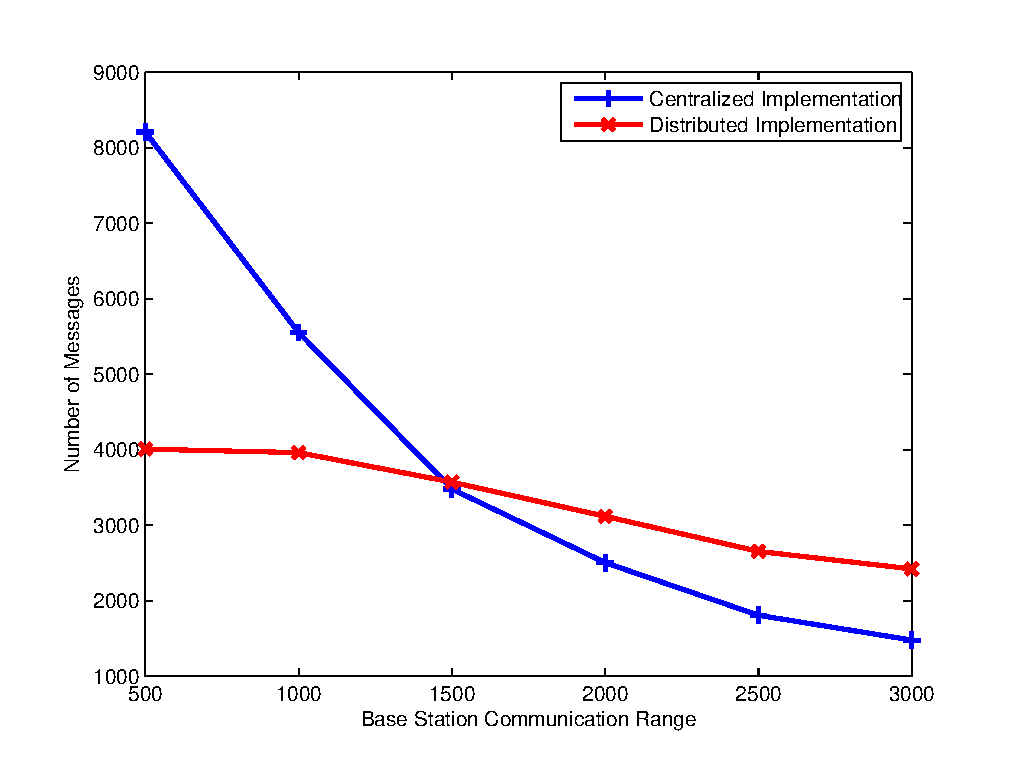
\includegraphics[width=0.6\columnwidth]{fig/RangeCompare}
  \caption[Effect of changing the base station range on code
  decomposition]{Changing the base station range changes the balance between the
  two decompositions.}
  \label{fig:RangeCompare}
\end{figure}

In the third deployment scenario, a high-gain antenna is added to the
base-station which increases the coverage of the base station and changes
the cost profile of the network.  Figure~\ref{fig:MainResult} shows that
adding the antenna reduces the cost of messages dramatically.  This cost
reduction is because the increased range allows all of the nodes to more
cheaply communicate with the base station.  However, this change affects
the centralized decomposition to a greater extent.  This is because all nodes in the
network use the base station link in the centralized implementation while
in the distributed implementation, only the nodes that can
opportunistically route through the base station to reduce messaging costs
to other nodes on the route will actually do so.  Increasing the base
station range increases the number of nodes that opportunistically route
through the base station, reducing messaging costs but not as dramatically
as in a centralized decomposition. Figure~\ref{fig:RangeCompare} shows
that for more then a 1500 meter range, the centralized implementation gives superior
performance. 

In this scenario, a centralized decomposition costs 1468 messages while the
distributed version costs 2472 messages. This is a reversal of the cost
trade-off in the previous scenario. Small changes to radio hardware can lead to
large changes in the cost profile of the target deployment. Redesigning a TinyOS
program to be efficient given this new cost profile would be difficult, but the
MacroLab framework makes this change automatically.

\subsubsection{Scenario 4: Additional Route} 
\begin{figure}
  \centering
  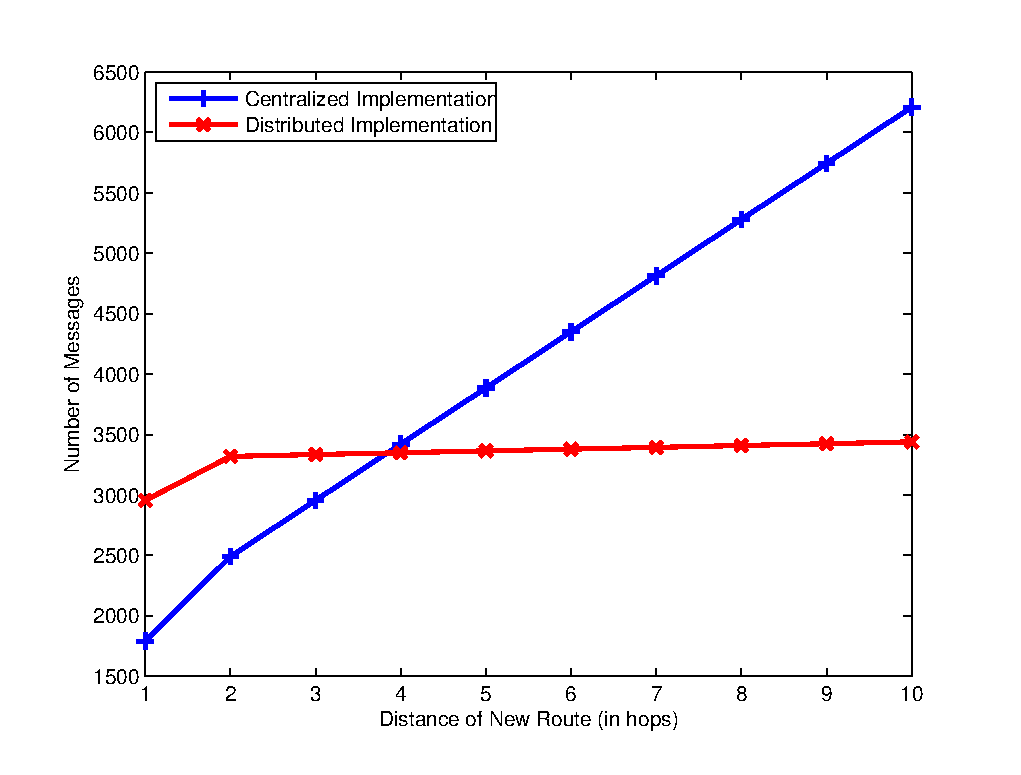
\includegraphics[width=0.6\columnwidth]{fig/MovingRoute}
  \caption[Effect of adding a route to code decomposition]{Adding a new route at
  various distances changes the balance between the two decompositions.}
  \label{fig:MovingRoute}
\end{figure}

In the fourth deployment scenario a route that runs from the main campus to a
new location 2500 meters away from the base station is added.
Figure~\ref{fig:MovingRoute} shows the distributed and centralized costs as a
function of the number of hops from the base station. As the number of hops
increases, the centralized decomposition must send messages farther to reach the
base station, while the cost of the distributed decomposition does not
change. Once this messaging cost to and from the base station exceeds the cost
of sending messages directly to the other nodes in the route, it is more
expensive to utilize the centralized implementation.

Figure~\ref{fig:MainResult} shows that at an additional 4000 meters, the
distributed version becomes more efficient than the centralized
decomposition. The centralized cost is 6210 and the distributed cost is 3439.
Because the new route is farther away from the base station, communication with
the base station becomes more expensive. This scenario demonstrates that small
changes to the network topology can cause large changes to the cost profile of
the target deployment.

\subsection{Accuracy of Static Cost Analyzer}
\label{sect:analysisAccuracy}
\begin{figure}
  \centering
  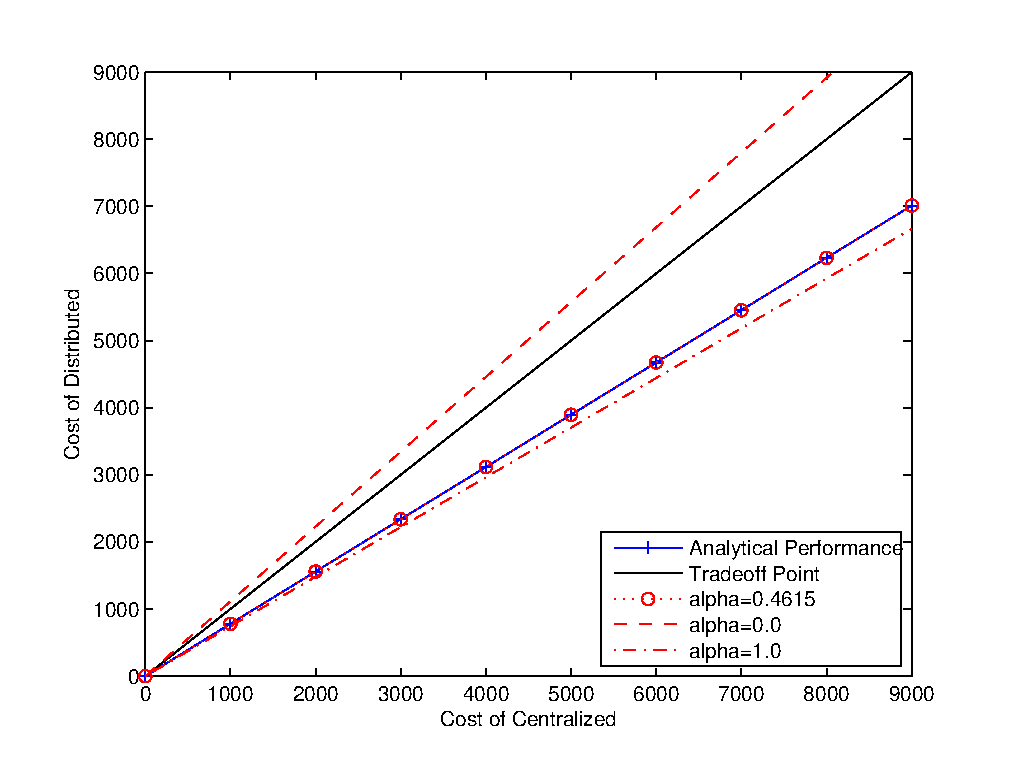
\includegraphics[width=0.6\columnwidth]{fig/Buses}
  \caption[Estimated and measured messaging costs]{Estimated and measured
  messaging costs. The parameter $\alpha$ is the ratio of buses on long routes
  versus those on all other routes. The actual distribution of bus detection
  events can change the true messaging cost within a narrow range around the
  statically estimated cost.  }
  \label{fig:Buses}
\end{figure}

The static cost analysis (Section~\ref{sect:staticCost}) can make
use of information about expected event frequency. For simple event-loop
MacroLab programs, the presence and quality of this event frequency
information is the determining factor in the accuracy of the analysis.
In the worst case, such information is not available. For the bus
tracking application, lacking any other information, the static analysis
assumes that each bus stop observes a bus event with the same frequency.
However, this is not necessarily true and there will be some
discrepancy between the cost estimated by the static analysis and the
actual cost of the decompositions. For example, if a larger percentage
of buses appear on very long routes, this will increase the cost of the
distributed decomposition relative to the static estimate. On the other
hand, if many buses appear on routes far from the base
station, this would increase the cost of the centralized decomposition.

Figure~\ref{fig:Buses} shows static estimated costs as well as dynamic measured
costs as the distribution of buses and therefore sensed events within the
network changes.  To highlight the differences between the centralized and
distributed implementations, the evaluation focuses on the longest routes. The
parameter $\alpha$ is defined as the ratio of buses on the long routes versus
those on all other routes.  The crossover point for centralized and distributed
message costs is represented by the $y=x$ line.  Ratios above the crossover line
will be optimally run as centralized applications, those below as distributed.
By computing the ratios for various scenarios, the effect of the change on the
total cost of the application, and whether it will cause a switch in the optimal
implementation, can be seen.  The bounds of the application are plotted by the
$\alpha = 0$ and $\alpha = 1$ lines, in which either all buses or no buses
appear on the longest routes. The static cost analysis algorithm is quite
accurate for this application and is not extremely sensitive to the assumptions
made about the frequency of events; it will only be incorrect with extremely
non-uniform event distributions.  In such cases, the run-time system can
dynamically monitor changes or errors in the cost profile of the target
deployment.  As shown in Figure~\ref{fig:System}, such dynamic cost information
can be fed back into the cost analyzer which can decide to reprogram the
network.

\section{Conclusions} \label{conclusions}
MacroLab's approach of {\em deployment-specific code decomposition} addresses a
central question in the area of Cyber-Physical Systems software design: should programs
be implemented in a centralized or distributed fashion?  Most early sensor
network research focused on ``{\em localized} algorithms -- where sensors only
interact with other sensors in a restricted vicinity, but nevertheless
collectively achieve a desired global objective''~\cite{Estrin}.  For
example, early object tracking applications argue that neighborhood
communication and local processing are necessary to efficiently filter false
positives~\cite{Whitehousea} and services like TAG use {\em
in-network aggregation} to calculate network statistics {\em en route} to
decrease message passing~\cite{Madden}.  More recently, several
architectures have proposed the use of centralized algorithms to control
distributed systems. {\em Marionette} allows the user to write a
centralized Python script to control all nodes in a
network~\cite{Whitehouseb}.  It argues that centralized algorithms are
easier to write and debug and that, once debugged, functionality can be {\em
migrated} to the sensor nodes for efficiency reasons if
necessary~\cite{Whitehouse}. The {\em Tenet}~\cite{Gnawali} architecture
takes a stronger stance by arguing that all application-specific code should
{\em always} execute on master devices while sensor nodes should be restricted
to a small set of predefined operations on locally-generated data. The rationale
here is to separate the application code from the networking code so that
changes in the application do not cause cascading changes to the networking
middleware.

MacroLab demonstrates that programs can actually be implemented in both a
centralized {\em and} a distributed fashion. The architectural question is
reframed from {\em where code should execute} to {\em how code should be
written}.  The central tenet of MacroLab's architecture is that all
application-specific logic should be contained in a macroprogram and all
distributed operations must be contained as libraries in the run-time system.
When code is written in this way: (1) the decomposer and the run-time system can
choose the manner of implementation that provides the best performance in terms
of cost metrics like bandwidth, power, and latency, and (2) the user is free to
write {\em deployment-independent} programs that are simple, robust, and easy to
understand.  In future work, new macrovector representations will be used to
decompose programs into many points on the spectrum between purely centralized
or purely distributed code, such as hierarchical or group-based data processing,
and in-network aggregation.
